\documentclass[11pt,a4paper]{article}
\usepackage[top=1.2cm,bottom=1.4cm,left=1.4cm,right=1.4cm]{geometry}
\usepackage[dvipsnames,svgnames,table]{xcolor}
\usepackage{tcolorbox}
\tcbuselibrary{skins,breakable,fitting}
\usepackage{booktabs}
\usepackage{array}
\usepackage{colortbl}
\usepackage{tabularx}
\usepackage{multicol}
\usepackage{amsmath}
\usepackage{amssymb}
\usepackage[T1]{fontenc}
\usepackage{lmodern}
\usepackage{tikz}
\usetikzlibrary{shapes.geometric,arrows.meta,positioning,shadows.blur,calc}
\usepackage{microtype}
\usepackage{graphicx}
\usepackage{enumitem}
\usepackage{fancyhdr}
\usepackage{parskip}
\usepackage{mdframed}

% ─── Colour palette ───────────────────────────────────────────────
\definecolor{Navy}   {HTML}{0D2137}
\definecolor{Royal}  {HTML}{1565C0}
\definecolor{SkyBg}  {HTML}{E3F2FD}
\definecolor{DOrange}{HTML}{BF360C}
\definecolor{LOrange}{HTML}{FFF3E0}
\definecolor{DGreen} {HTML}{1B5E20}
\definecolor{LGreen} {HTML}{E8F5E9}
\definecolor{Teal}   {HTML}{00695C}
\definecolor{LTeal}  {HTML}{E0F2F1}
\definecolor{Purple} {HTML}{4A148C}
\definecolor{LPurple}{HTML}{F3E5F5}
\definecolor{DRed}   {HTML}{C62828}
\definecolor{LRed}   {HTML}{FFEBEE}
\definecolor{Amber}  {HTML}{F57F17}
\definecolor{LAmber} {HTML}{FFFDE7}
\definecolor{DGray}  {HTML}{424242}
\definecolor{LGray}  {HTML}{F5F5F5}
\definecolor{MGray}  {HTML}{9E9E9E}
\definecolor{Indigo} {HTML}{283593}

% ─── Page style ───────────────────────────────────────────────────
\setlength{\parindent}{0pt}
\setlength{\parskip}{4pt}
\pagestyle{fancy}
\fancyhf{}
\fancyhead[L]{\small\color{MGray}\textbf{VANI} --- Results \& Methods Summary \quad|\quad Vishal Sharma, Gaurav Agarwal, Sanket Sharma}
\fancyhead[R]{\small\color{MGray}IIT Indore · IEEE INDISCON 2026}
\fancyfoot[C]{\small\color{MGray}\thepage}
\renewcommand{\headrulewidth}{0.3pt}
\setlength{\headheight}{14pt}

% ─── Helper: coloured rule ────────────────────────────────────────
\newcommand{\crule}[3]{\textcolor{#1}{\rule{#2}{#3}}}

% ─── tcolorbox shortcuts ─────────────────────────────────────────
\newtcolorbox{banner}[2]{enhanced,colback=#1,colframe=#1,arc=6pt,
  boxrule=0pt,left=10pt,right=10pt,top=7pt,bottom=7pt,
  fontupper=\bfseries\color{white}\large, title={},#2}

\newtcolorbox{kpibox}[2]{enhanced,colback=#1,colframe=#2,arc=8pt,
  boxrule=2pt,left=8pt,right=8pt,top=8pt,bottom=8pt,
  shadow={2pt}{-2pt}{0pt}{black!18},center upper,#2}

\newtcolorbox{infobox}[2]{enhanced,colback=#1,colframe=#2,arc=5pt,
  boxrule=1.2pt,left=7pt,right=7pt,top=6pt,bottom=6pt}

\newtcolorbox{stageblue}[0]{enhanced,colback=SkyBg,colframe=Royal,arc=4pt,
  boxrule=1pt,left=6pt,right=6pt,top=5pt,bottom=5pt}

\newtcolorbox{stageorange}[0]{enhanced,colback=LOrange,colframe=DOrange,arc=4pt,
  boxrule=1.5pt,left=6pt,right=6pt,top=5pt,bottom=5pt}

% ══════════════════════════════════════════════════════════════════
\begin{document}

% ── TITLE BANNER ──────────────────────────────────────────────────
\begin{tcolorbox}[enhanced,colback=Navy,colframe=Navy,arc=8pt,
  boxrule=0pt,left=14pt,right=14pt,top=12pt,bottom=10pt]
\centering
{\fontsize{24}{28}\selectfont\bfseries\color{white}
  VANI: Voice Analysis \& Neural Intelligence}\\[5pt]
{\large\color{SkyBg}
  Offline Multilingual Spoken Language Pipeline for Indian Border-Region Languages}\\[3pt]
{\normalsize\color{MGray}
  Vishal Sharma · Gaurav Agarwal · Sanket Sharma
  \quad\textbullet\quad IIT Indore
  \quad\textbullet\quad IEEE INDISCON 2026}
\end{tcolorbox}

\vspace{5pt}

% ── KPI ROW ───────────────────────────────────────────────────────
\noindent
\begin{minipage}[t]{0.245\textwidth}
\begin{tcolorbox}[enhanced,colback=LGreen,colframe=DGreen,arc=8pt,boxrule=2pt,
  left=6pt,right=6pt,top=7pt,bottom=7pt,shadow={2pt}{-2pt}{0pt}{black!15},center upper]
{\fontsize{32}{36}\selectfont\bfseries\color{DGreen}96.7\%}\\[1pt]
{\small\bfseries\color{DGreen}LangID Accuracy}\\
{\footnotesize\color{DGray}Hindi \& Punjabi\\end-to-end (30 each)}
\end{tcolorbox}
\end{minipage}\hfill
\begin{minipage}[t]{0.245\textwidth}
\begin{tcolorbox}[enhanced,colback=SkyBg,colframe=Royal,arc=8pt,boxrule=2pt,
  left=6pt,right=6pt,top=7pt,bottom=7pt,shadow={2pt}{-2pt}{0pt}{black!15},center upper]
{\fontsize{32}{36}\selectfont\bfseries\color{Royal}+19.9\,pp}\\[1pt]
{\small\bfseries\color{Royal}MMS-LID Gain}\\
{\footnotesize\color{DGray}Macro-avg LangID\\50.8\% $\to$ 70.7\%}
\end{tcolorbox}
\end{minipage}\hfill
\begin{minipage}[t]{0.245\textwidth}
\begin{tcolorbox}[enhanced,colback=LOrange,colframe=DOrange,arc=8pt,boxrule=2pt,
  left=6pt,right=6pt,top=7pt,bottom=7pt,shadow={2pt}{-2pt}{0pt}{black!15},center upper]
{\fontsize{32}{36}\selectfont\bfseries\color{DOrange}100\%}\\[1pt]
{\small\bfseries\color{DOrange}Translation Done}\\
{\footnotesize\color{DGray}120 Indic files\\pa / hi / ur / ne}
\end{tcolorbox}
\end{minipage}\hfill
\begin{minipage}[t]{0.245\textwidth}
\begin{tcolorbox}[enhanced,colback=LPurple,colframe=Purple,arc=8pt,boxrule=2pt,
  left=6pt,right=6pt,top=7pt,bottom=7pt,shadow={2pt}{-2pt}{0pt}{black!15},center upper]
{\fontsize{32}{36}\selectfont\bfseries\color{Purple}{$<$}8\,GB}\\[1pt]
{\small\bfseries\color{Purple}Peak RAM}\\
{\footnotesize\color{DGray}Consumer laptop\\no GPU, fully offline}
\end{tcolorbox}
\end{minipage}

\vspace{5pt}

% ── PROBLEM STATEMENT ─────────────────────────────────────────────
\begin{tcolorbox}[enhanced,colback=LRed,colframe=DRed,arc=5pt,boxrule=1.5pt,
  left=9pt,right=9pt,top=7pt,bottom=7pt]
\textbf{\color{DRed}\large The Core Problem --- Silent Language Misidentification}\\[5pt]
\begin{tabular}{@{}p{3.5cm}p{5.5cm}p{6.5cm}@{}}
\textbf{Audio input:} & Punjabi recording \texttt{sent\_1.wav} & \\[2pt]
\textbf{Whisper alone:} & Returns \texttt{hi} (Hindi) at 0.690 conf. & \textcolor{DRed}{\textbf{$\times$ Wrong language, wrong script}} \\[2pt]
\textbf{FastText confirms:} & Also returns Hindi at 0.891 conf. & \textcolor{DRed}{\textbf{$\times$ Both text sources agree --- both wrong}} \\[2pt]
\textbf{MMS-LID (audio):} & Returns \texttt{pa} (Punjabi) at 1.000 conf. & \textcolor{DGreen}{\textbf{\checkmark{} Audio evidence overrides both}} \\[2pt]
\textbf{VANI output:} & \texttt{pa} --- correct language \& script & \textcolor{DGreen}{\textbf{\checkmark{} Routed to correct translation model}} \\
\end{tabular}\\[5pt]
\small This failure is not a quirk of one recording. Whisper's training data contains orders of magnitude more Hindi than Punjabi. The two languages are phonologically close. Whisper picks the majority-class language every time. FastText reads the wrong-script transcript and confirms the same error. Only an audio-grounded source that bypasses the ASR decoder can break this loop --- and that is what MMS-LID provides.
\end{tcolorbox}

% ══════════════════════════════════════════════════════════════════
\newpage

% ── METHOD: PIPELINE ──────────────────────────────────────────────
\begin{tcolorbox}[enhanced,colback=Navy,colframe=Navy,arc=5pt,boxrule=0pt,
  left=10pt,right=10pt,top=5pt,bottom=5pt]
{\large\bfseries\color{white}METHOD --- The 10-Stage Processing Pipeline}
\end{tcolorbox}

\vspace{5pt}

% Pipeline diagram
\begin{center}
\scalebox{0.78}{%
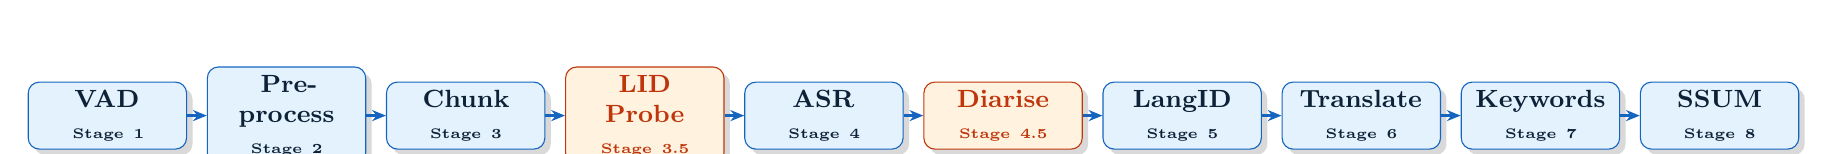
\begin{tikzpicture}[
  box/.style={draw=Royal,rectangle,rounded corners=4pt,fill=SkyBg,
    font=\small\bfseries\color{Navy},text width=1.8cm,minimum height=0.85cm,
    align=center,inner sep=3pt,drop shadow={opacity=0.3}},
  nov/.style={draw=DOrange,rectangle,rounded corners=4pt,fill=LOrange,
    font=\small\bfseries\color{DOrange},text width=1.8cm,minimum height=0.85cm,
    align=center,inner sep=3pt,drop shadow={opacity=0.3}},
  arr/.style={-{Stealth[length=5pt,width=4pt]},thick,draw=Royal},
  node distance=0.25cm
]
\node[box](n1){VAD\\{\tiny Stage 1}};
\node[box,right=of n1](n2){Pre-\\process\\{\tiny Stage 2}};
\node[box,right=of n2](n3){Chunk\\{\tiny Stage 3}};
\node[nov,right=of n3](n35){\textbf{LID}\\Probe\\{\tiny Stage 3.5}};
\node[box,right=of n35](n4){ASR\\{\tiny Stage 4}};
\node[nov,right=of n4](n45){\textbf{Diarise}\\{\tiny Stage 4.5}};
\node[box,right=of n45](n5){LangID\\{\tiny Stage 5}};
\node[box,right=of n5](n6){Translate\\{\tiny Stage 6}};
\node[box,right=of n6](n7){Keywords\\{\tiny Stage 7}};
\node[box,right=of n7](n8){SSUM\\{\tiny Stage 8}};
\draw[arr](n1)--(n2);\draw[arr](n2)--(n3);\draw[arr](n3)--(n35);
\draw[arr](n35)--(n4);\draw[arr](n4)--(n45);\draw[arr](n45)--(n5);
\draw[arr](n5)--(n6);\draw[arr](n6)--(n7);\draw[arr](n7)--(n8);
\end{tikzpicture}%
}% end scalebox

\vspace{3pt}
\small\textcolor{Royal}{$\blacksquare$} Standard stages \quad
\textcolor{DOrange}{$\blacksquare$} \textbf{Novel stages} (3.5 \& 4.5 --- not present in vanilla ASR pipelines)
\end{center}

\vspace{5pt}

% Stage descriptions --- 2 columns
\begin{multicols}{2}

\begin{stageblue}
\textbf{\color{Royal}Stage 1 --- Voice Activity Detection}\\
\small Silero-VAD strips silence and non-speech before ASR sees anything. Without this, Whisper was transcribing radio carrier hiss as coherent sentences. Peak RAM: $<$0.2\,GB.
\end{stageblue}

\vspace{4pt}

\begin{stageblue}
\textbf{\color{Royal}Stage 2 --- Channel Preprocessing}\\
\small 4th-order Butterworth bandpass (300--3400\,Hz) removes sub-bass rumble and HF noise outside the voice range. Stationary spectral subtraction removes constant carrier hiss. RMS normalisation to $-$20\,dBFS.
\end{stageblue}

\vspace{4pt}

\begin{stageblue}
\textbf{\color{Royal}Stage 3 --- Audio Chunking}\\
\small Audio is split at VAD speech boundaries, not fixed time windows. Fixed windows were clipping the first word of utterances often enough to measurably hurt WER.
\end{stageblue}

\vspace{4pt}

\begin{stageorange}
\textbf{\color{DOrange}$\bigstar$ Stage 3.5 --- Pre-ASR LID Probe (Novel)}\\
\small MMS-LID-256 classifies language from the raw waveform \textit{before} Whisper receives anything. Predictions above 0.65 confidence go directly to the Whisper decoder as a script hint, forcing it to write Nastaliq for Urdu or Devanagari for Hindi/Nepali from chunk one --- not after ASR fails first.\\[3pt]
\textbf{Why it matters:} Breaks the feedback loop where Whisper and FastText both commit to the same wrong answer before Stage 5 can correct them.
\end{stageorange}

\columnbreak

\begin{stageblue}
\textbf{\color{Royal}Stage 4 --- ASR: Whisper large-v3-turbo (int8)}\\
\small Quantised to int8 via CTranslate2. Active RAM $<$2\,GB with $<$1\% accuracy loss. Two critical decoder flags: \texttt{condition\_on\_previous\_text=False} kills repetition loops (radio noise triggers them), \texttt{no\_speech\_threshold=0.70} drops non-speech segments. Without the filter, carrier hiss was transcribed as Portuguese and Icelandic during development.
\end{stageblue}

\vspace{4pt}

\begin{stageorange}
\textbf{\color{DOrange}$\bigstar$ Stage 4.5 --- Speaker Diarization (Novel)}\\
\small MFCC features (13 coefficients + $\Delta$ + $\Delta\Delta$ = 39 dimensions) fed into Ward-linkage agglomerative clustering. $k$ selected 1--4 by within-cluster elbow. \textbf{No pre-trained speaker embedding required.} Speaker labels travel with each segment through LangID, translation, and SSUM, so the final report separates who said what.
\end{stageorange}

\vspace{4pt}

\begin{stageblue}
\textbf{\color{Royal}Stage 5 --- LangID Ensemble (Three Sources)}\\
\small Confidence-weighted vote of Whisper + FastText + MMS-LID with Unicode script-block hard overrides. Full detail on next page.
\end{stageblue}

\vspace{4pt}

\begin{stageblue}
\textbf{\color{Royal}Stage 6 --- Neural Machine Translation}\\
\small NLLB-200-distilled-600M (2.4\,GB RAM) covers all 15 target languages. Dogri (\texttt{doi}) only: IndicTrans2-indic-en-1B fallback. Models load on demand and are explicitly freed (\texttt{del model; gc.collect()}) before the next stage.
\end{stageblue}

\vspace{4pt}

\begin{stageblue}
\textbf{\color{Royal}Stages 7 \& 8 --- Keywords \& SSUM}\\
\small \textbf{Stage 7:} Configurable threat-indicator dictionary (exact + fuzzy) raises alert level \texttt{CLEAR $\to$ LOW $\to$ MEDIUM $\to$ HIGH $\to$ CRITICAL}. \textbf{Stage 8:} Rule-based 5W extractor targets NATO callsigns, MGRS grid refs, unit designators, time expressions. Optional Qwen2.5-1.5B int4 LLM refines fields.
\end{stageblue}

\end{multicols}

\vspace{4pt}

% Hardware footprint table
\begin{tcolorbox}[enhanced,colback=LAmber,colframe=Amber,arc=5pt,boxrule=1.2pt,
  left=8pt,right=8pt,top=6pt,bottom=6pt]
\textbf{\color{Amber}Hardware Footprint --- Sequential Loading, No Co-Residency}\\[4pt]
\begin{tabularx}{\linewidth}{@{}lrrX@{}}
\textbf{Stage} & \textbf{Model} & \textbf{Parameters} & \textbf{Peak RAM}\\
\midrule
VAD / Prep & Silero-VAD & --- & $<$0.2\,GB \\
ASR (S4) & Whisper lv3-turbo CT2 int8 & 809\,M & $\sim$1.9\,GB \\
LID Probe (S3.5) & MMS-LID-256 & 150\,M & $\sim$0.6\,GB \\
Text LID & FastText lid.176.bin & --- & $\sim$0.9\,GB \\
Translation & NLLB-200-distilled-600M & 600\,M & $\sim$2.4\,GB \\
SSUM opt. & Qwen2.5-1.5B int4 & 1.5\,B & $\sim$1.1\,GB \\
\midrule
\multicolumn{3}{@{}l}{\textbf{Total (peak, all stages):}} & \textbf{$<$7.8\,GB --- consumer laptop, no GPU, fully offline}\\
\end{tabularx}
\end{tcolorbox}

% ══════════════════════════════════════════════════════════════════
\newpage

% ── METHOD: LangID ENSEMBLE ───────────────────────────────────────
\begin{tcolorbox}[enhanced,colback=Purple,colframe=Purple,arc=5pt,boxrule=0pt,
  left=10pt,right=10pt,top=5pt,bottom=5pt]
{\large\bfseries\color{white}METHOD --- Three-Source Language Identification Ensemble (Stage 5)}
\end{tcolorbox}

\vspace{5pt}

\noindent
\begin{minipage}[t]{0.32\textwidth}
\begin{tcolorbox}[enhanced,colback=SkyBg,colframe=Royal,arc=6pt,boxrule=2pt,
  left=7pt,right=7pt,top=7pt,bottom=7pt,shadow={2pt}{-2pt}{0pt}{black!12}]
\centering{\bfseries\color{Royal}Source 1}\\[3pt]
{\large\color{Navy}\textbf{Whisper}}\\
{\small\color{DGray}Encoder Probability}\\[5pt]
\rule{\linewidth}{0.4pt}\\[4pt]
\small\raggedright
\textbf{Input:} Audio waveform (via ASR decoder)\\[3pt]
\textbf{Strength:} Works well for well-resourced languages --- English, Mandarin, Hindi.\\[3pt]
\textbf{Weakness:} Gravitates to training-data majority. Punjabi $\to$ Hindi. Nepali $\to$ Gujarati. No mechanism to disagree with itself.
\end{tcolorbox}
\end{minipage}\hfill
\begin{minipage}[t]{0.32\textwidth}
\begin{tcolorbox}[enhanced,colback=LTeal,colframe=Teal,arc=6pt,boxrule=2pt,
  left=7pt,right=7pt,top=7pt,bottom=7pt,shadow={2pt}{-2pt}{0pt}{black!12}]
\centering{\bfseries\color{Teal}Source 2}\\[3pt]
{\large\color{Teal}\textbf{FastText}}\\
{\small\color{DGray}Character N-gram Classifier}\\[5pt]
\rule{\linewidth}{0.4pt}\\[4pt]
\small\raggedright
\textbf{Input:} ASR transcript text\\[3pt]
\textbf{Strength:} Very fast. Covers 176 languages. Strong on clean text.\\[3pt]
\textbf{Weakness:} Inherits every Whisper error. Wrong-script Devanagari for Punjabi $\to$ FastText says Hindi. Both text-based sources share the same failure mode.
\end{tcolorbox}
\end{minipage}\hfill
\begin{minipage}[t]{0.32\textwidth}
\begin{tcolorbox}[enhanced,colback=LOrange,colframe=DOrange,arc=6pt,boxrule=2pt,
  left=7pt,right=7pt,top=7pt,bottom=7pt,shadow={2pt}{-2pt}{0pt}{black!12}]
\centering{\bfseries\color{DOrange}Source 3 $\bigstar$ KEY}\\[3pt]
{\large\color{DOrange}\textbf{MMS-LID-256}}\\
{\small\color{DGray}Raw Waveform Classifier}\\[5pt]
\rule{\linewidth}{0.4pt}\\[4pt]
\small\raggedright
\textbf{Input:} Raw audio waveform only\\[3pt]
\textbf{Strength:} Never reads the transcript. Classifies purely from acoustic phoneme patterns. Can disagree with both text-based sources and be right.\\[3pt]
\textbf{Adds:} 150\,M params, $\sim$0.6\,GB RAM. Worth it: +19.9\,pp.
\end{tcolorbox}
\end{minipage}

\vspace{6pt}

\begin{tcolorbox}[enhanced,colback=LPurple,colframe=Purple,arc=5pt,boxrule=1.5pt,
  left=9pt,right=9pt,top=7pt,bottom=7pt]
\textbf{\color{Purple}Voting Rules \& Unicode Script-Block Overrides}\\[4pt]
\begin{tabular}{@{}p{4cm}p{12cm}@{}}
\textbf{Script check (runs first):} &
$\bullet$ $>$20\% Gurmukhi chars (U+0A00--U+0A7F) $\to$ \textbf{force Punjabi} (Gurmukhi is unique to Punjabi in South Asian writing --- zero ambiguity)\\
& $\bullet$ $>$20\% Arabic/Nastaliq $\to$ narrow candidate set to \{ur, ks, sd, ps, fa, ar\} before voting\\[4pt]
\textbf{3/3 unanimous:} & Score $\times$1.10 (10\% confidence boost --- highest certainty)\\[2pt]
\textbf{2/3 majority:} & Average the two agreeing scores\\[2pt]
\textbf{0/3 agreement:} & Top-scoring source wins, $\times$0.85 penalty\\[4pt]
\textbf{Score below 0.60:} & Tagged \texttt{uncertain}; \texttt{LOW\_LANG\_CONFIDENCE} flag travels with output through all downstream stages\\
\end{tabular}
\end{tcolorbox}

\vspace{6pt}

\begin{tcolorbox}[enhanced,colback=LAmber,colframe=Amber,arc=5pt,boxrule=1.5pt,
  left=9pt,right=9pt,top=7pt,bottom=7pt]
\textbf{\color{Amber}Why Stage 3.5 (Pre-ASR Probe) is Critical --- Not Just Stage 5}\\[4pt]
\begin{tabular}{@{}p{2cm}p{6.5cm}p{6.5cm}@{}}
& \textbf{Without Stage 3.5} & \textbf{With Stage 3.5}\\
\midrule
\textbf{Urdu} & Whisper writes \textbf{Devanagari}; Arabic-script filter finds nothing; LangID 57--58\% & Whisper writes \textbf{Nastaliq}; Arabic-script filter activates; \textbf{LangID 70.0\% (+12\,pp)}\\[3pt]
\textbf{Nepali} & Devanagari output; Gurmukhi filter irrelevant; MMS-LID outvoted & Script hint reinforces MMS-LID; fewer hallucinations\\[3pt]
\textbf{Mandarin} & Already 99.3\% without hint (CJK script is unambiguous) & No change needed\\
\end{tabular}
\end{tcolorbox}

% ══════════════════════════════════════════════════════════════════
\newpage

% ── RESULTS: ABLATION ─────────────────────────────────────────────
\begin{tcolorbox}[enhanced,colback=DGreen,colframe=DGreen,arc=5pt,boxrule=0pt,
  left=10pt,right=10pt,top=5pt,bottom=5pt]
{\large\bfseries\color{white}RESULTS --- LangID Ablation Study (1,475 FLEURS Samples)}
\end{tcolorbox}

\vspace{5pt}

\begin{tcolorbox}[enhanced,colback=LGray,colframe=MGray!50,arc=4pt,boxrule=0.7pt,
  left=7pt,right=7pt,top=5pt,bottom=5pt]
\small\textbf{Method:} Four progressively complete configurations on 1,475 FLEURS test samples (295 per language, 5 languages: Punjabi, Hindi, Urdu, Nepali, Mandarin). \texttt{language\_hint=None} held fixed throughout to isolate the LangID ensemble from Stage 3.5 conditioning. 95\% CIs from 10,000-resample bootstrap.
\end{tcolorbox}

\vspace{5pt}

{\small
\begin{tabular}{lrrrrr>{\bfseries}r}
\toprule
\rowcolor{Navy}
\color{white}\textbf{Configuration} &
\color{white}\textbf{Punjabi (pa)} &
\color{white}\textbf{Hindi (hi)} &
\color{white}\textbf{Urdu (ur)} &
\color{white}\textbf{Nepali (ne)} &
\color{white}\textbf{Mandarin (zh)} &
\color{white}\textbf{Overall}\\
\midrule
Whisper only     & \cellcolor{LRed}0.0\% [0,0]   & \cellcolor{LGreen}85.1\% [81,89] & \cellcolor{LAmber}58.0\% [52,63] & \cellcolor{LRed}0.0\% [0,0]   & \cellcolor{LGreen}100.0\% [100,100] & \cellcolor{LRed}48.6\%\\
+FastText        & \cellcolor{LRed}0.0\% [0,0]   & \cellcolor{LGreen}85.1\% [81,89] & \cellcolor{LAmber}57.3\% [52,63] & \cellcolor{LAmber}12.5\% [9,16]& \cellcolor{LGreen}99.3\% [98,100]  & \cellcolor{LRed}50.8\%\\
\rowcolor{LGreen!60}
+MMS-LID         & 91.9\% [89,95] & 85.1\% [81,89] & 58.0\% [53,64] & 19.3\% [15,24] & 99.3\% [98,100] & 70.7\%\\
\rowcolor{SkyBg}
\textbf{Full VANI} & \textbf{91.2\%} & \textbf{85.1\%} & \textbf{58.0\%} & \textbf{19.3\%} & \textbf{99.3\%} & \textbf{70.6\%}\\
\bottomrule
\end{tabular}
}

\vspace{6pt}

% Visual bar chart using rule
\noindent\textbf{\color{DGreen}Visual: Macro-Average LangID Accuracy by Configuration}\\[4pt]
\begin{tabular}{@{}l@{\hspace{4pt}}l@{\hspace{6pt}}l@{}}
Whisper only & \crule{DRed}{3.89cm}{0.45cm} & \small 48.6\% \\[3pt]
+FastText    & \crule{Amber}{4.06cm}{0.45cm} & \small 50.8\%\quad{\color{Amber}(+2.2\,pp from FastText)}\\[3pt]
+MMS-LID     & \crule{DGreen}{5.66cm}{0.45cm} & \small 70.7\%\quad{\color{DGreen}\textbf{(+19.9\,pp from MMS-LID --- the key jump)}}\\[3pt]
Full VANI    & \crule{Royal}{5.65cm}{0.45cm} & \small 70.6\%\quad{($-$0.1\,pp from script override)}\\
\end{tabular}

\vspace{6pt}

\noindent
\begin{minipage}[t]{0.32\textwidth}
\begin{tcolorbox}[enhanced,colback=LRed,colframe=DRed,arc=5pt,boxrule=1.5pt,
  left=6pt,right=6pt,top=6pt,bottom=6pt]
\centering{\Large\bfseries\color{DRed}+2.2\,pp}\\
{\small\bfseries FastText adds little}\\[4pt]
\small\raggedright FastText reads the ASR transcript. When Whisper writes the wrong script, FastText reads that wrong text and arrives at the same wrong answer. Both text-based sources share exactly the same failure mode.
\end{tcolorbox}
\end{minipage}\hfill
\begin{minipage}[t]{0.32\textwidth}
\begin{tcolorbox}[enhanced,colback=LGreen,colframe=DGreen,arc=5pt,boxrule=1.5pt,
  left=6pt,right=6pt,top=6pt,bottom=6pt]
\centering{\Large\bfseries\color{DGreen}+19.9\,pp}\\
{\small\bfseries MMS-LID is decisive}\\[4pt]
\small\raggedright MMS-LID operates on raw audio --- independent of the ASR transcript. It breaks the text-source feedback loop. Punjabi: \textbf{0\% to 91.9\%}. Nepali: 0\% to 19.3\%. One acoustic vote changes the outcome.
\end{tcolorbox}
\end{minipage}\hfill
\begin{minipage}[t]{0.32\textwidth}
\begin{tcolorbox}[enhanced,colback=SkyBg,colframe=Royal,arc=5pt,boxrule=1.5pt,
  left=6pt,right=6pt,top=6pt,bottom=6pt]
\centering{\Large\bfseries\color{Royal}$-$0.1\,pp}\\
{\small\bfseries Script override: edge case}\\[4pt]
\small\raggedright Minimal aggregate impact. Earns its place: when MMS-LID confidence is borderline but Gurmukhi character share is unambiguous, the script rule catches misses the ensemble would leave on the table.
\end{tcolorbox}
\end{minipage}

\vspace{5pt}

\begin{tcolorbox}[enhanced,colback=LOrange,colframe=DOrange,arc=6pt,boxrule=2pt,
  left=9pt,right=9pt,top=7pt,bottom=7pt]
\textbf{\color{DOrange}\large Punjabi: 0\% $\to$ 91.9\% --- The Binary Difference MMS-LID Makes}\\[4pt]
Without MMS-LID: \textbf{every single one} of the 295 Punjabi samples was routed as Hindi. Whisper outputs Devanagari; FastText reads Devanagari and confirms Hindi. Both text-based sources agree on the wrong answer with high confidence.\\[4pt]
With MMS-LID: \textbf{91.9\% of Punjabi samples} (CI: [89--95\%]) are correctly identified. MMS-LID classifies from acoustic phoneme patterns in the raw waveform --- Punjabi phonology is distinct enough from Hindi for an audio model to separate them even when the ASR transcript cannot.\\[4pt]
\textbf{This is not a marginal improvement. Without MMS-LID, Punjabi is completely broken. With it, the system is operational.}
\end{tcolorbox}

% ══════════════════════════════════════════════════════════════════
\newpage

% ── RESULTS: INTEGRATED PIPELINE ──────────────────────────────────
\begin{tcolorbox}[enhanced,colback=DOrange,colframe=DOrange,arc=5pt,boxrule=0pt,
  left=10pt,right=10pt,top=5pt,bottom=5pt]
{\large\bfseries\color{white}RESULTS --- Integrated Pipeline: 180 FLEURS Samples, All 10 Stages Active}
\end{tcolorbox}

\vspace{5pt}

\begin{tcolorbox}[enhanced,colback=LGray,colframe=MGray!50,arc=4pt,boxrule=0.7pt,
  left=7pt,right=7pt,top=4pt,bottom=4pt]
\small\textbf{Method:} 30 FLEURS test clips per language across 6 languages (\texttt{en\_us}, \texttt{pa\_in}, \texttt{hi\_in}, \texttt{ur\_pk}, \texttt{ne\_np}, \texttt{cmn\_hans\_cn}), clipped to 2--20\,s. Full 10 stages, Stage 3.5 hint enabled.
\end{tcolorbox}

\vspace{5pt}

{\small
\begin{tabular}{lrrrrrl}
\toprule
\rowcolor{Navy}
\color{white}\textbf{Language} &
\color{white}\textbf{LangID} &
\color{white}\textbf{Transcribed} &
\color{white}\textbf{WER} &
\color{white}\textbf{CER} &
\color{white}\textbf{RTF (CPU)} &
\color{white}\textbf{Translation}\\
\midrule
\rowcolor{LGreen}English (en)   & 30/30 (100\%)        & 29/30 & --- & --- & 2.91$\times$ & skip (English)\\
\rowcolor{LGreen}Punjabi (pa)   & \textbf{29/30 (96.7\%)} & 29/30 & N/A$^\dagger$ & N/A$^\dagger$ & 4.57$\times$ & \textbf{100\%}\\
\rowcolor{LGreen}Hindi (hi)     & \textbf{29/30 (96.7\%)} & 30/30 & \textbf{46.2\%} & \textbf{32.4\%} & 4.11$\times$ & \textbf{100\%}\\
\rowcolor{LAmber}Urdu (ur)      & 21/30 (70.0\%)       & 19/30 & 74.4\% & 63.2\% & 8.98$\times$ & \textbf{100\%}\\
\rowcolor{LRed}Nepali (ne)    & 19/30 (63.3\%)       & 8/30  & N/A$^\ddagger$ & N/A$^\ddagger$ & 7.00$\times$ & \textbf{100\%}\\
\rowcolor{LGreen}Mandarin (zh)  & 29/30 (96.7\%)       & 27/30 & ---  & ---  & 6.40$\times$ & skip\\
\bottomrule
\multicolumn{7}{l}{\footnotesize\textcolor{DGreen}{$\blacksquare$} $\geq$90\%\quad\textcolor{Amber}{$\blacksquare$} 70--89\%\quad\textcolor{DRed}{$\blacksquare$} $<$70\%}\\
\multicolumn{7}{l}{\footnotesize $\dagger$ Script mismatch: Whisper outputs Devanagari; FLEURS Punjabi references in Gurmukhi --- WER not comparable.}\\
\multicolumn{7}{l}{\footnotesize $\ddagger$ Whisper hallucinated European text on low-confidence Nepali audio (mean confidence 0.187).}\\
\end{tabular}
}

\vspace{5pt}

\noindent
\begin{minipage}[t]{0.32\textwidth}
\begin{tcolorbox}[enhanced,colback=LGreen,colframe=DGreen,arc=5pt,boxrule=1.5pt,
  left=6pt,right=6pt,top=6pt,bottom=6pt]
\textbf{\color{DGreen}Hindi \& Punjabi --- 96.7\%}\\[3pt]
\small One failure each. Both cases: audio with heavy Urdu/Persian loanwords that push the ensemble toward Urdu. No model fix --- this is a vocabulary overlap problem.
\end{tcolorbox}
\end{minipage}\hfill
\begin{minipage}[t]{0.32\textwidth}
\begin{tcolorbox}[enhanced,colback=LAmber,colframe=Amber,arc=5pt,boxrule=1.5pt,
  left=6pt,right=6pt,top=6pt,bottom=6pt]
\textbf{\color{Amber}Urdu --- 70.0\%}\\[3pt]
\small 9 failures: 8/9 FastText returned \texttt{unknown}. Arabic-script filter rescued 3. Remaining 6 had too little Nastaliq content. Stage 3.5 contributes +12\,pp over ablation.
\end{tcolorbox}
\end{minipage}\hfill
\begin{minipage}[t]{0.32\textwidth}
\begin{tcolorbox}[enhanced,colback=LRed,colframe=DRed,arc=5pt,boxrule=1.5pt,
  left=6pt,right=6pt,top=6pt,bottom=6pt]
\textbf{\color{DRed}Nepali --- 63.3\%}\\[3pt]
\small 11 failures = Whisper hallucinations (mean conf. 0.187). MMS-LID voted correctly in 4/11 failures and was overruled 2-to-1 each time.
\end{tcolorbox}
\end{minipage}

\vspace{5pt}

% Robustness table
\textbf{\color{Teal}\large Robustness under Channel Degradations (120 Indic Samples)}

\vspace{3pt}
{\small
\begin{tabular}{lrrrr}
\toprule
\rowcolor{Navy}
\color{white}\textbf{Condition} &
\color{white}\textbf{Whisper only} &
\color{white}\textbf{+FastText} &
\color{white}\textbf{+MMS-LID} &
\color{white}\textbf{Full VANI}\\
\midrule
Clean            & 38.3\% & 40.0\% & 53.3\% & \cellcolor{LGreen}\textbf{69.2\%}\\
Bandpass 300--3400\,Hz & 30.0\% & 30.0\% & 42.5\% & \cellcolor{LAmber}\textbf{54.2\%}\\
AWGN 10\,dB SNR  & 35.8\% & 40.8\% & 55.8\% & \cellcolor{LGreen}\textbf{70.8\%}\\
AWGN 0\,dB SNR   & 22.5\% & 22.5\% & 30.8\% & \cellcolor{LAmber}\textbf{42.5\%}\\
MP3 16\,kbps     & 28.3\% & 28.3\% & 41.7\% & \cellcolor{LAmber}\textbf{52.5\%}\\
\bottomrule
\end{tabular}
}

\vspace{3pt}
\begin{tcolorbox}[enhanced,colback=LTeal,colframe=Teal,arc=4pt,boxrule=1pt,
  left=7pt,right=7pt,top=5pt,bottom=5pt]
\small MMS-LID added +8 to +15\,pp in \textit{every} condition --- audio-grounded ID holds as channel quality drops; transcript-based methods do not. Under bandpass and MP3, FastText gained exactly 0\,pp over Whisper-only. At 0\,dB SNR, Full VANI still reached \textbf{42.5\%} vs.\ 22.5\% for Whisper-only. No rank reversals across any noise level.
\end{tcolorbox}

\vspace{5pt}

% Comparison with baselines
\textbf{\color{Purple}\large Comparison with Published Baselines}

\vspace{3pt}
\noindent
\begin{minipage}[t]{0.48\textwidth}
\begin{tcolorbox}[enhanced,colback=LGray,colframe=MGray,arc=4pt,boxrule=0.8pt,
  left=7pt,right=7pt,top=5pt,bottom=5pt]
\small\textbf{Published (general-domain, balanced benchmarks):}\\[3pt]
\begin{tabular}{@{}lll@{}}
FastText & Text only & $>$97\%\\
MMS-LID & Audio only & $>$90\%\\
Whisper & Audio+Text & $\sim$95\%\\
\end{tabular}
\end{tcolorbox}
\end{minipage}\hfill
\begin{minipage}[t]{0.48\textwidth}
\begin{tcolorbox}[enhanced,colback=SkyBg,colframe=Royal,arc=4pt,boxrule=1.5pt,
  left=7pt,right=7pt,top=5pt,bottom=5pt]
\small\textbf{Ours (border-region languages, 180 samples):}\\[3pt]
\begin{tabular}{@{}ll@{}}
Whisper-only baseline & 35.8\%\\
\textbf{Full VANI Ensemble} & \textbf{81.7\%}\\
\end{tabular}\\[3pt]
\textbf{The 59\,pp gap is the test set.} Punjabi and Nepali near zero under Whisper-only, included because they are the operationally relevant languages.
\end{tcolorbox}
\end{minipage}

% ══════════════════════════════════════════════════════════════════
\newpage

% ── SAMPLE OUTPUT + TAKEAWAYS ─────────────────────────────────────
\begin{tcolorbox}[enhanced,colback=Navy,colframe=Navy,arc=5pt,boxrule=0pt,
  left=10pt,right=10pt,top=5pt,bottom=5pt]
{\large\bfseries\color{white}RESULTS --- Sample SSUM Output \& Key Takeaways}
\end{tcolorbox}

\vspace{5pt}

% SSUM sample
\begin{tcolorbox}[enhanced,colback=LAmber,colframe=Amber,arc=6pt,boxrule=1.5pt,
  left=9pt,right=9pt,top=7pt,bottom=7pt]
\textbf{\color{Amber}Live SSUM Report --- \texttt{sent\_1.wav} (Punjabi audio, 7.0\,s)}\\[5pt]
\begin{tabular}{@{}p{3.5cm}p{12cm}@{}}
\textbf{Language detected:} & \texttt{pa} --- confidence 0.993, \texttt{hi}$\to$\texttt{pa} MMS-LID override applied\\[2pt]
\textbf{Who:} & Mukhi (SPEAKER\_0), National Council NCVAT\\[2pt]
\textbf{What:} & Decision to establish National Council NCVAT\\[2pt]
\textbf{Where:} & Not identified\\[2pt]
\textbf{When:} & Not identified\\[2pt]
\textbf{Alert level:} & \texttt{CLEAR}\\[2pt]
\textbf{Quality flags:} & None\\
\end{tabular}\\[5pt]
\small This report was generated from an audio recording where Whisper (0.690) and FastText (0.891) both returned Hindi. MMS-LID returned Punjabi at 1.000 confidence, overrode both, routed to the correct translation model, and the 5W extractor produced a clean structured report. Zero analyst intervention needed.
\end{tcolorbox}

\vspace{6pt}

\noindent
\begin{minipage}[t]{0.48\textwidth}
\begin{tcolorbox}[enhanced,colback=LGreen,colframe=DGreen,arc=6pt,boxrule=2pt,
  left=8pt,right=8pt,top=7pt,bottom=7pt,shadow={2pt}{-2pt}{0pt}{black!12}]
\textbf{\color{DGreen}\large What Works}\\[4pt]
\begin{itemize}[leftmargin=*,itemsep=2pt,topsep=0pt]
  \item \textbf{96.7\% LangID} for Hindi and Punjabi end-to-end
  \item \textbf{100\% translation completion} across 120 Indic files (pa/hi/ur/ne) --- no stage failures
  \item \textbf{+19.9\,pp from MMS-LID} --- every percentage point attributable to one design decision
  \item Punjabi \textbf{0\% $\to$ 91.9\%} with MMS-LID; \textbf{0\% $\to$ 96.7\%} end-to-end with Stage 3.5
  \item Fits in \textbf{$<$8\,GB RAM}, any consumer laptop, fully offline
  \item Audio-based ID is \textbf{rank-stable} across all five degradation conditions
  \item Speaker diarization with \textbf{no pre-trained embedding} required
  \item 81.7\% vs.\ 35.8\% Whisper-only on the same test set
\end{itemize}
\end{tcolorbox}
\end{minipage}\hfill
\begin{minipage}[t]{0.48\textwidth}
\begin{tcolorbox}[enhanced,colback=LRed,colframe=DRed,arc=6pt,boxrule=2pt,
  left=8pt,right=8pt,top=7pt,bottom=7pt,shadow={2pt}{-2pt}{0pt}{black!12}]
\textbf{\color{DRed}\large Remaining Gaps \& Fixes}\\[4pt]
\begin{itemize}[leftmargin=*,itemsep=2pt,topsep=0pt]
  \item \textbf{Urdu at 70.0\%} --- depends on Stage 3.5 hint; Arabic-script filter blind without Nastaliq output
  \item \textbf{Nepali at 63.3\%} --- shares Devanagari with Hindi; character counts useless; Nepali morphological postposition rule would break the 2-to-1 tie
  \item \textbf{Hindi WER 46.2\%} --- Whisper transcription quality, not a LangID failure
  \item \textbf{One Punjabi ensemble failure} (cv-pa.mp3) --- Whisper hallucinated Icelandic; MMS-LID outvoted 2-to-1
  \item FLEURS is \textbf{read speech} --- conversational, code-switched, and field recording performance untested
\end{itemize}
\end{tcolorbox}
\end{minipage}

\vspace{6pt}

\begin{tcolorbox}[enhanced,colback=SkyBg,colframe=Royal,arc=6pt,boxrule=2pt,
  left=9pt,right=9pt,top=8pt,bottom=8pt,shadow={2pt}{-2pt}{0pt}{black!12}]
\textbf{\color{Royal}\large The Central Design Insight}\\[5pt]
Language identification must draw on more than ASR-derived evidence.\\[4pt]
FastText adds +2.2\,pp because it reads the same Whisper output that caused the error. MMS-LID adds +19.9\,pp because it reads the raw audio waveform --- independent of the ASR transcript. \textbf{One architectural decision. Visible in every table, every degradation condition, every noise level.}\\[4pt]
\begin{center}
\begin{tabular}{ccccc}
\large\bfseries\color{DRed}35.8\% & \large$\xrightarrow{\text{+FastText}}$ & \large\bfseries\color{Amber}50.8\% & \large$\xrightarrow{\text{+MMS-LID}}$ & \large\bfseries\color{DGreen}81.7\%\\
{\footnotesize Whisper only} & & {\footnotesize +2.2\,pp} & & {\footnotesize \textbf{+19.9\,pp}}\\
\end{tabular}
\end{center}
\end{tcolorbox}

\vspace{6pt}

\begin{tcolorbox}[enhanced,colback=LPurple,colframe=Purple,arc=5pt,boxrule=1.5pt,
  left=9pt,right=9pt,top=7pt,bottom=7pt]
\textbf{\color{Purple}Next Steps}\\[4pt]
\begin{tabular}{@{}p{4cm}p{11.5cm}@{}}
\textbf{Nepali morphology:} & Postposition-based rule to break the Devanagari tie with Hindi without touching acoustic models\\[2pt]
\textbf{Bengali \& Pashto:} & Eastern and north-western border corridors --- natural extension of the existing pipeline\\[2pt]
\textbf{Code-switched recordings:} & Current evaluation entirely on clean read speech; field recordings will expose real-world degradation\\[2pt]
\textbf{Diarization evaluation:} & Formal DER measurement requires annotated multispeaker data\\[2pt]
\textbf{GPU deployment:} & RTF drops from 3--9$\times$ to below 0.3$\times$ --- enables real-time operation at the edge\\
\end{tabular}
\end{tcolorbox}

\end{document}
